\documentclass[UTF8]{ctexart}
% \documentclass[12pt]{report}
\usepackage{ctex}
\usepackage{setspace}
\usepackage{graphicx}
\usepackage{float}
\usepackage{geometry}
\usepackage{makecell}
\usepackage[table,xcdraw]{xcolor}
\usepackage{listings}
\geometry{a4paper,scale=0.8}
\setCJKmainfont{SimSun}
\renewcommand{\normalsize}{\fontsize{12pt}{15pt}\selectfont}
\setstretch{1.0}

\begin{document}


\title{智能计算芯片导论期末课程设计报告——基于RISCV向量扩展指令集的VPU设计}
\maketitle
\begin{center}
	22307130445 贾梓越
\end{center}

\section{设计目标}

\section{设计架构}

\section{设计实现}

\section{测试结果}
测试输入为三个8*8的矩阵,一个存储在向量缓存中,两个存储在标量缓存中,计算矩阵的乘加运算,测试数据为随机生成,如下:
\begin{equation}
Matrix_1
=
\left[
\begin{array}{cccccccc}
    -69 & 95  & 73  & -55 & 17  & 32  & -16 & 24  \\
    100 & -93 & 56  & 41  & 47  & 83  & -69 & 4   \\
    77  & -83 & -26 & -78 & -14 & -27 & 75  & 1   \\
    -54 & 62  & 88  & 13  & -18 & 39  & 0   & 97  \\
    -12 & 85  & 58  & -80 & 44  & 53  & -99 & 66  \\
    -37 & 7   & 99  & 25  & -61 & 18  & 55  & -92 \\
    -70 & 49  & -34 & 81  & 60  & -47 & 28  & -85 \\
    -2  & 100 & -59 & 36  & -77 & 72  & 11  & -63 
\end{array}
\right]
\end{equation}

\begin{equation}
Matrix_2
=
\left[
\begin{array}{cccccccc}
    -88 & 14  & 67  & -99 & 53  & 80  & -41 & 22  \\
    -7  & 91  & -62 & 38  & 100 & -56 & 19  & -84 \\
    -35 & 60  & 27  & -90 & 45  & 8   & -30 & 73  \\
    59  & -13 & 92  & -75 & 31  & -68 & 85  & -24 \\
    -96 & 70  & 2   & 99  & -50 & 63  & -17 & 44  \\
    81  & -28 & 54  & -61 & 12  & 97  & -79 & 6   \\
    -58 & 35  & 100 & -87 & 29  & -32 & 76  & -9  \\
    40  & -95 & 21  & 65  & -73 & 58  & -12 & 90
\end{array}
\right]
\end{equation}

\begin{equation}
Matrix_3
=
\left[
\begin{array}{cccccccc}
    81 & -44 & 56 & -90 &  13 & 67 & -38 &  72\\
   -99 &  35 &-73 &  40 &  86 &-65 &  17 &  33\\
    27 & -88 & 62 & -41 &  19 & 77 & -56 &  84\\
   -13 &  95 &-22 &  59 & -80 & 36 &  48 & -71\\
    61 & -24 & 79 & -92 &  55 & 12 & -38 &  70\\
   -47 &  81 &-66 &  28 & -35 & 99 & -21 &  10\\
    53 & -60 & 44 & -85 &  72 &-18 &  25 & -97\\
   -31 &  67 &-49 &  90 & -76 & 38 &  63 & -29
\end{array}
\right]
\end{equation}

理论结果为

\begin{equation}
\left[
\begin{array}{cccccccc}
    2536  &  10184 & -12880 &  10589 &  4754  & -370   & -6590  &  467   \\
   -1416  & -6030  &  15437 & -15656 & -3770  &  24255 & -16693 &  16696 \\
   -15013 & -4803  &  8524  & -8827  & -5310  &  10138 & -2581  &  7361  \\
    10759 & -1475  &  195   &  1010  &  1908  &  339   & -2034  &  7817  \\
    2223  &  3924  & -17353 &  19132 & -1204  &  15105 & -19722 &  7905  \\
    1614  &  11706 &  6412  & -24730 &  15511 & -13354 &  5683  & -6116  \\
   -2752  &  14897 & -2553  &  6538  &  5696  & -20747 &  17572 & -15723 \\
    13700 &  4095  & -1153  & -10369 &  17911 & -10515 &  4088  & -22369
\end{array}
\right]
\end{equation}

测试用的汇编代码如下:
\lstset{
 columns=fixed,       
 numbers=left,                                        % 在左侧显示行号
 numberstyle=\tiny\color{gray},                       % 设定行号格式
 frame=none,                                          % 不显示背景边框
 backgroundcolor=\color[RGB]{245,245,244},            % 设定背景颜色
 keywordstyle=\color[RGB]{40,40,255},                 % 设定关键字颜色
 numberstyle=\footnotesize\color{darkgray},           
 commentstyle=\it\color[RGB]{0,96,96},                % 设置代码注释的格式
 stringstyle=\rmfamily\slshape\color[RGB]{128,0,0},   % 设置字符串格式
 showstringspaces=false,                              % 不显示字符串中的空格
 language=c++,                                        % 设置语言
}
\begin{lstlisting}
    // line1
    MOV     R1,       0x0     // R1 = 0x0
    VLOAD  VR2,  R0,  0x8     // VR2 = Matrix_3[0][:]
    VMAC   VR3,  R2,  VR2, 1  // VR3 = VR2

    LOAD    R2,  R1,  0x0     // R2 = Matrix_1[0][0]
    VLOAD  VR2,  R0,  0x0     // VR2 = Matrix_2[0][:]
    VMAC   VR3,  R2,  VR2, 0  // VR3 = R2 * VR2 + VR3

    LOAD    R2,  R1,  0x1     // R2 = Matrix_1[0][1]
    VLOAD  VR2,  R0,  0x1     // VR2 = Matrix_2[1][:]
    VMAC   VR3,  R2,  VR2, 0  // VR3 = R2 * VR2 + VR3

    LOAD    R2,  R1,  0x2     // R2 = Matrix_1[0][2]
    VLOAD  VR2,  R0,  0x2     // VR2 = Matrix_2[2][:]
    VMAC   VR3,  R2,  VR2, 0  // VR3 = R2 * VR2 + VR3

    LOAD    R2,  R1,  0x3     // R2 = Matrix_1[0][3]
    VLOAD  VR2,  R0,  0x3     // VR2 = Matrix_2[3][:]
    VMAC   VR3,  R2,  VR2, 0  // VR3 = R2 * VR2 + VR3

    LOAD    R2,  R1,  0x4     // R2 = Matrix_1[0][4]
    VLOAD  VR2,  R0,  0x4     // VR2 = Matrix_2[4][:]
    VMAC   VR3,  R2,  VR2, 0  // VR3 = R2 * VR2 + VR3

    LOAD    R2,  R1,  0x5     // R2 = Matrix_1[0][5]
    VLOAD  VR2,  R0,  0x5     // VR2 = Matrix_2[5][:]
    VMAC   VR3,  R2,  VR2, 0  // VR3 = R2 * VR2 + VR3

    LOAD    R2,  R1,  0x6     // R2 = Matrix_1[0][6]
    VLOAD  VR2,  R0,  0x6     // VR2 = Matrix_2[6][:]
    VMAC   VR3,  R2,  VR2, 0  // VR3 = R2 * VR2 + VR3

    LOAD    R2,  R1,  0x7     // R2 = Matrix_1[0][7]
    VLOAD  VR2,  R0,  0x7     // VR2 = Matrix_2[7][:]
    VMAC   VR3,  R2,  VR2, 0  // VR3 = R2 * VR2 + VR3

    MOV     R3,       0x10    // R3 = 0x10(after matrix3)
    VSTORE  R3,  VR2          // store VR2 to VectorDCM[16]

    // line2
    MOV     R1,       0x8     // R1 = 0x8
    VLOAD  VR2,  R0,  0x9     // VR2 = Matrix_3[1][:]
    VMAC   VR3,  R2,  VR2, 1  // VR3 = VR2

    LOAD    R2,  R1,  0x0     // R2 = Matrix_1[1][0]
    VLOAD  VR2,  R0,  0x0     // VR2 = Matrix_2[0][:]
    VMAC   VR3,  R2,  VR2, 0  // VR3 = R2 * VR2 + VR3

    LOAD    R2,  R1,  0x1     // R2 = Matrix_1[1][1]
    VLOAD  VR2,  R0,  0x1     // VR2 = Matrix_2[1][:]
    VMAC   VR3,  R2,  VR2, 0  // VR3 = R2 * VR2 + VR3

    LOAD    R2,  R1,  0x2     // R2 = Matrix_1[1][2]
    VLOAD  VR2,  R0,  0x2     // VR2 = Matrix_2[2][:]
    VMAC   VR3,  R2,  VR2, 0  // VR3 = R2 * VR2 + VR3

    LOAD    R2,  R1,  0x3     // R2 = Matrix_1[1][3]
    VLOAD  VR2,  R0,  0x3     // VR2 = Matrix_2[3][:]
    VMAC   VR3,  R2,  VR2, 0  // VR3 = R2 * VR2 + VR3

    LOAD    R2,  R1,  0x4     // R2 = Matrix_1[1][4]
    VLOAD  VR2,  R0,  0x4     // VR2 = Matrix_2[4][:]
    VMAC   VR3,  R2,  VR2, 0  // VR3 = R2 * VR2 + VR3

    LOAD    R2,  R1,  0x5     // R2 = Matrix_1[1][5]
    VLOAD  VR2,  R0,  0x5     // VR2 = Matrix_2[5][:]
    VMAC   VR3,  R2,  VR2, 0  // VR3 = R2 * VR2 + VR3

    LOAD    R2,  R1,  0x6     // R2 = Matrix_1[1][6]
    VLOAD  VR2,  R0,  0x6     // VR2 = Matrix_2[6][:]
    VMAC   VR3,  R2,  VR2, 0  // VR3 = R2 * VR2 + VR3

    LOAD    R2,  R1,  0x7     // R2 = Matrix_1[1][7]
    VLOAD  VR2,  R0,  0x7     // VR2 = Matrix_2[7][:]
    VMAC   VR3,  R2,  VR2, 0  // VR3 = R2 * VR2 + VR3

    MOV     R3,       0x11    // R3 = 0x11(after matrix3)
    VSTORE  R3,  VR2          // store VR2 to VectorDCM[17]

    ...

    // line8
    MOV     R1,       0x38     // R1 = 0x38
    VLOAD  VR2,  R0,  0xf     // VR2 = Matrix_3[7][:]
    VMAC   VR3,  R2,  VR2, 1  // VR3 = VR2

    LOAD    R2,  R1,  0x0     // R2 = Matrix_1[7][0]
    VLOAD  VR2,  R0,  0x0     // VR2 = Matrix_2[0][:]
    VMAC   VR3,  R2,  VR2, 0  // VR3 = R2 * VR2 + VR3

    LOAD    R2,  R1,  0x1     // R2 = Matrix_1[7][1]
    VLOAD  VR2,  R0,  0x1     // VR2 = Matrix_2[1][:]
    VMAC   VR3,  R2,  VR2, 0  // VR3 = R2 * VR2 + VR3

    LOAD    R2,  R1,  0x2     // R2 = Matrix_1[7][2]
    VLOAD  VR2,  R0,  0x2     // VR2 = Matrix_2[2][:]
    VMAC   VR3,  R2,  VR2, 0  // VR3 = R2 * VR2 + VR3

    LOAD    R2,  R1,  0x3     // R2 = Matrix_1[7][3]
    VLOAD  VR2,  R0,  0x3     // VR2 = Matrix_2[3][:]
    VMAC   VR3,  R2,  VR2, 0  // VR3 = R2 * VR2 + VR3

    LOAD    R2,  R1,  0x4     // R2 = Matrix_1[7][4]
    VLOAD  VR2,  R0,  0x4     // VR2 = Matrix_2[4][:]
    VMAC   VR3,  R2,  VR2, 0  // VR3 = R2 * VR2 + VR3

    LOAD    R2,  R1,  0x5     // R2 = Matrix_1[7][5]
    VLOAD  VR2,  R0,  0x5     // VR2 = Matrix_2[5][:]
    VMAC   VR3,  R2,  VR2, 0  // VR3 = R2 * VR2 + VR3

    LOAD    R2,  R1,  0x6     // R2 = Matrix_1[7][6]
    VLOAD  VR2,  R0,  0x6     // VR2 = Matrix_2[6][:]
    VMAC   VR3,  R2,  VR2, 0  // VR3 = R2 * VR2 + VR3

    LOAD    R2,  R1,  0x7     // R2 = Matrix_1[7][7]
    VLOAD  VR2,  R0,  0x7     // VR2 = Matrix_2[7][:]
    VMAC   VR3,  R2,  VR2, 0  // VR3 = R2 * VR2 + VR3

    MOV     R3,       0x17    // R3 = 0x17(after matrix3)
    VSTORE  R3,  VR2          // store VR2 to VectorDCM[23]

\end{lstlisting}

计算的结果存放在VectorDCM中,程序运行结束后将计算结果读出并在tcl窗口中打印,结果如下:

\begin{figure}[htbp]
    \centering
    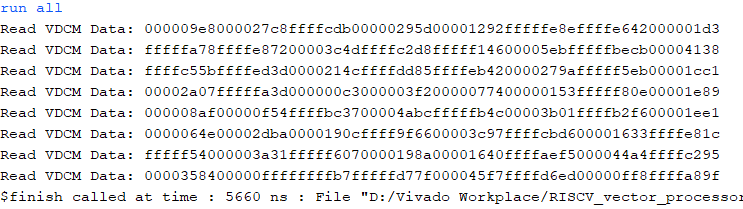
\includegraphics[width=16cm]{pic/matrix_result.png}
    \caption{m32n8k16矩阵乘法任务分配示意图}
\end{figure}

对应的十进制数与理想结果相同,表明处理器可以正常工作。

\end{document}